\chapter{GSM移动通信系统}
\section{GSM总体结构}
\subsection{系统结构}
\begin{figure}[htbp]
	\centering
	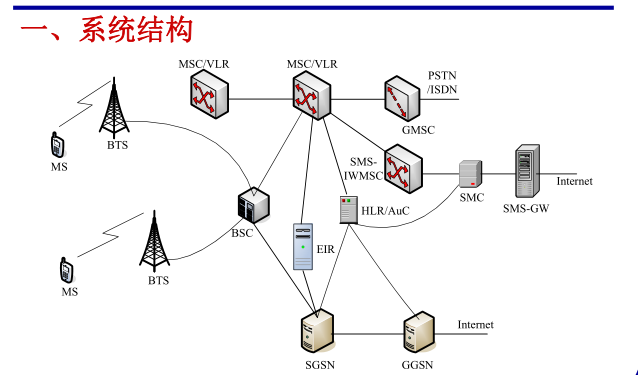
\includegraphics[width=0.7\linewidth]{figures/screenshot003}
	\caption{}
	\label{fig:screenshot003}
\end{figure}
GSM网络由MS,BSS,NSS三部分组成。
\begin{itemize}
	\item BSS:包括BTS和BSC
	\item NSS:包括核心网功能实体
	\begin{itemize}
		\item 电路域,MSC/VLR,GMSC,SMS-IWMSC、SMC、SMS-GW、HLR/AuC和EIR
		\item 分组域,SGSN,GGSN。
	\end{itemize}
\end{itemize}
\subsection{协议栈和接口}
\begin{figure}[H]
	\centering
	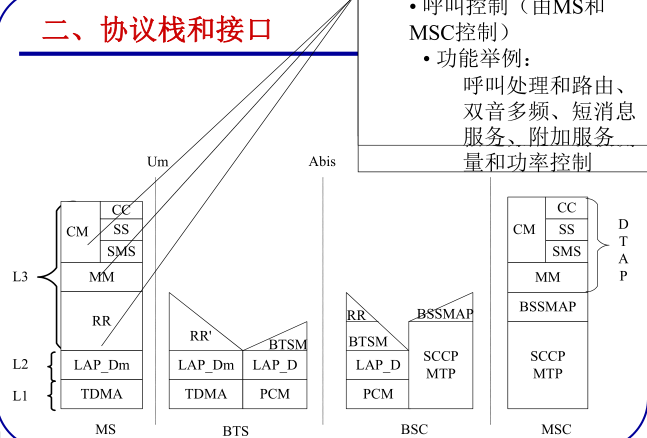
\includegraphics[width=0.7\linewidth]{figures/screenshot004}
	\caption{}
	\label{fig:screenshot004}
\end{figure}
\begin{enumerate}
	\item Um接口,是MS和BTS的空中接口,共三层(网络、数据链路和物理层)
	\begin{enumerate}
		\item CM,连接管理
		\item MM,移动性管理,包括位置登记和呼叫传递,在MS和MSC中实现。
		\item RR,无线资源管理。
	\end{enumerate}
	\item Abis,BTS和BSC之间的接口。
	\item A,BSC和MSC之间的接口。
\end{enumerate}
\section{无线信道}
中国地区使用900/1800MHz。其中以900为主,1800不是到处都有。GSM采用FDD工作方式,在900MHz时,双工收发间隔是45MHz,在1800MHz双工收发间隔为905Hz。
一般地,\textbf{基站使用高频部分,补偿上下功率不平衡问题。}\\
在划分的上下行对称频段,按照\textbf{200kHz}间隔划分载波,每个载波采用TDMA方式,划分8个时隙(TS0-TS7),8个时隙共占用4.615ms。\\
载频间隔为0.2Hz,频道序号为n,则上下两频段中序号为n的载频可用下式计算:
\begin{gather}\label{key}
	\text{上行} f_{ul} = F_{ul0} +0.2n \\
	\text{下行} f_{dl} = F_{dl0} + 0.2n
\end{gather}
\subsection{干扰载波比}
\textbf{定义:}波干扰保护比C/I就是指接收到的希望信号
电平与非希望信号电平的比值。\\
GSM采用\textbf{高斯最小频移键控(GMSK)}、
\subsection{频率复用方式}
区群:将相邻若干的小区形成一个单元,在该单元内,所有小区不允许使用相同频率,且这种单元能无缝覆盖GSM业务提供去,单元之间频率符用。\\
小区个数:$ N= i^2 + ij+j^2 $
\begin{itemize}
	\item 模拟蜂窝采用7小区,采用全向天线。
	\item GSM,采用4小区或者3小区,采用扇区天线。
	\item 采用3小区使,同频小区距离较小,采用跳频技术来躲避同频干扰。
\end{itemize}
\subsubsection{4*3和3*3的频点配置}
\begin{figure}[H]
	\centering
	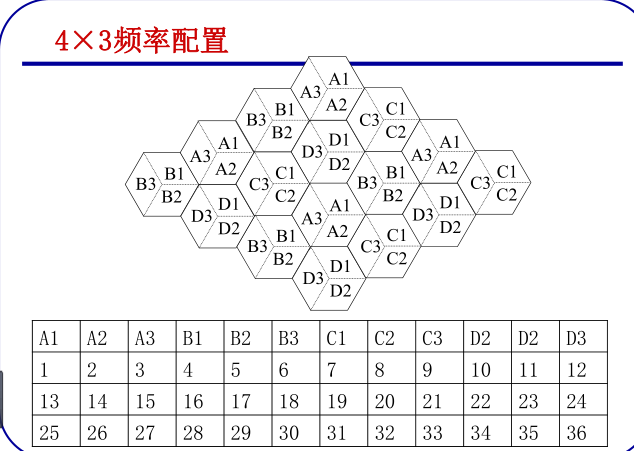
\includegraphics[width=0.7\linewidth]{figures/screenshot005}
	\caption{}
	\label{fig:screenshot005}
\end{figure}
\begin{figure}[H]
	\centering
	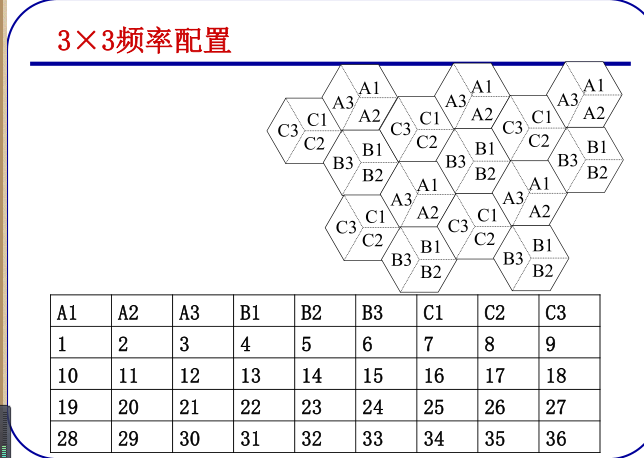
\includegraphics[width=0.7\linewidth]{figures/screenshot006}
	\caption{}
	\label{fig:screenshot006}
\end{figure}
为了提高系统容量
\begin{enumerate}
	\item 提升频率复用系数,即减少单个小区个数,使得复用次数增多,不过同频干扰增大。
	\item 小区分裂,减少原基站的覆盖半径,通
	过增加新基站来覆盖由于原基站覆盖半径减小而
	形成的盲区。
	\begin{figure}[tbph]
		\centering
		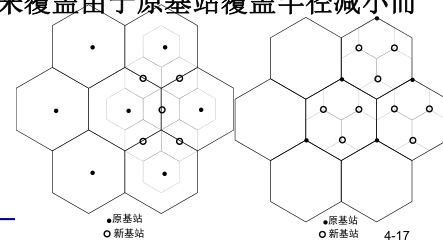
\includegraphics[width=0.7\linewidth]{figures/screenshot007}
		\caption{}
		\label{fig:screenshot007}
	\end{figure}
	基站布置方式有中心激励(天线采用全向天线)和顶点激励(天线采用扇区天线),两种布置方式的覆盖面积和基站个数均相同。
\end{enumerate}
\subsection{无线帧结构}
GSM 采用 TDMA 多址方式,在每载波上按时域
划分为 TS0 ~ TS7 共8 8 个时隙,时隙按 4.615ms 周期
性的重复,每个时隙即是一个物理信道。\\
超高帧--超帧--复帧--TDMA。
\textbf{MS占用上下行频率的时隙号相同,但上行时隙相对于下行时隙延后3个时隙时间。},原因
\begin{itemize}
	\item MS的收发信需要天线双工器来回倒换(对于只有一个天线的MS来说),倒换需要一定的时间。
	\item MS处于随机移动状态,它与BS之间的距离和位置随机变化,为了防止在不同位置使用相同频率的MS发射的时隙在到达BS的时候出现重叠的情况,离BS远的MS应当适当提前它的发射时刻,TA(时间提前量)。
\end{itemize}
\subsection{逻辑信道}
\begin{figure}[tbph]
	\centering
	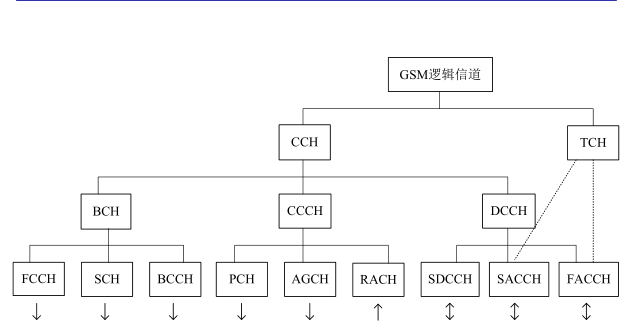
\includegraphics[width=0.7\linewidth]{figures/screenshot008}
	\caption{}
	\label{fig:screenshot008}
\end{figure}
\subsubsection{TCH}
传送语音数据和低速数据业务数据。
\begin{table}[htbp]
	\begin{tabular}{|c|c|c|}
		\hline 
		速度类型 & 语音编码速率 & 信道编码速率 \\ 
		\hline 
		全速率 & 13kb/s & 22.8kb/s \\ 
		\hline 
		半速率 & 6.5kb/s & 11.4kb/s \\ 
		\hline 
	\end{tabular} 	
\end{table}
\subsubsection{CCH}
传送信令数据以及短分组数据(短消息)。
\begin{description}
	\item[BCH(广播控制信道)] 一点对多点的下行控制信道;传送的内容主要使\textbf{移动台入网}和\textbf{呼叫建立}所需的有关信息。
	\begin{enumerate}
		\item 频率校正信道(FCCH),用于MS的频率矫正。
		\item 同步信道(SCH),传送基站识别码(BSIC,MS可以区分使用相同频率的不同基站,BS也可识别是否是连接到自身的MS),传送TDMA帧号(FN)。
		\item 广播控制信道(BCCH),MS由此获取各种系统参数(位置区识别LAI);同时,BS以\textbf{最强且恒定}公里吧发射该信道,MS通过检测该信道的信号质量作为越区切换判决用。
	\end{enumerate}
	\item [CCCH(公共控制信道)]双向控制信道,用于\textbf{呼叫接续}阶段传输链路连接所需的控制信令。
	\begin{enumerate}
		\item 寻呼信道PCH,用于寻呼移动台。在寻呼信道上,可以组呼多个MS,通过\textbf{TMSI},区分不同的MS。
		\item 随机接入信道(RACH),\textbf{上行},用于移动台提出入网申请,请求分配\textbf{SDCCH}。
		\item 接入允许信道AGCH,用于入网应答,分配一条SDCCH。
	\end{enumerate}
	\item [DCCH专用控制信道],双向,由基站分给某一特定的移动台专用
	\begin{enumerate}
		\item 独立专用控制信道SDCCH,用于在分配TCH之前接续过程中传送系统信令,用于传递位置登记、鉴权、呼叫建立、\textbf{短消息}等信令信息。经过鉴权确认后,在分配TCH。
		\item 慢速辅助控制信道SACCH
		\begin{itemize}
			\item 与SDCCH联用,构成SACCH-C,用于\textbf{周期性}传递MS对当前服务基站及周边基站信号的测量报告。
			\item 与TCH联用,构成SACCH-H,用于在\textbf{通话过程中},传递MS对当前基站和周边基站的测量报告,用于网络判决MS是否需要越区切换。以及TA下发,功率调整下发。
		\end{itemize}
		\item 快速辅助控制信道FACCG,与TCH联用。越区切换判决后,使用FACCH发送越区切换指令。
	\end{enumerate}
\end{description}
\begin{figure}[H]
	\centering
	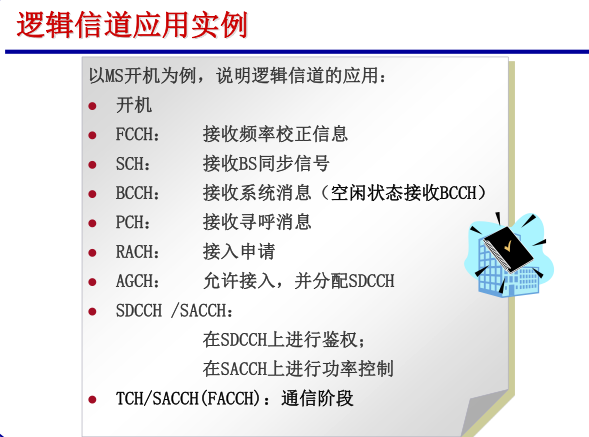
\includegraphics[width=0.7\linewidth]{figures/screenshot009}
	\caption{}
	\label{fig:screenshot009}
\end{figure}
\subsection{时隙格式}
GSM,8时隙,时隙宽度0.577ms,包含156.25bit。
\begin{description}
	\item[频率校正突发] 
	\item [同步突发]
	\item[  接入突发, (AB)] , 脉冲序列 。 用于
	RACH , 在 MS 初始接入时 , 利用接入突发传送信道
	请求消息。由保护期长度,可计算小区覆盖半径。
	\begin{figure}[H]
		\centering
		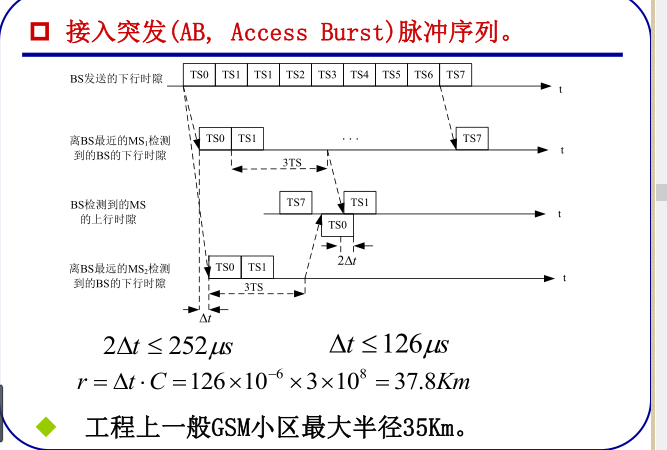
\includegraphics[width=0.7\linewidth]{figures/screenshot010}
		\caption{}
		\label{fig:screenshot010}
	\end{figure}
	\item[常规突发] 用于业务信道和专用控制信道。对于 BCCH 、 PCH 、 AGCH 、 SDCCH 、 SACCH 和 FACCH
	信道 , 采用 LAPDm 协议
\end{description}
\subsection{交织}
对于全速率TCH,GSM手机将20ms的模拟话音数据编码成260个比特(所以全速率话音速率为13kb/s),经过卷积编码等最终输出456bit。然后进行\textbf{块内和块间交织}。
\begin{description}
	\item[块内交织] 分为8个小块,每个小块456/8=57bit。
	\item[块间交织] 相邻两块数据进行二次交织,来自两个不同的57bit数据放入常规突发中。
\end{description}
\subsection{逻辑信道与物理信道映射}
对于多载频的情况下,系统会划分出主载频和副载频\textbf{,主载频上}的 TS0 和 TS1 用于映射控制信道,\textbf{主载频上的其余时隙和副载频上的所有时隙用于
映射业务信道}。
\subsubsection{BCH,CCCH}
对于\textbf{上行链路}, TS0 只用于 MS 的接入(RACH),即 51 个
TDMA(TS0) 帧用于随机接入信道。
\subsubsection{SDCCH、SACCH-C}
下行链路TS1用于映射专用控制信道。
\subsubsection{TCH}
复诊含有26个TDMA帧。
\begin{description}
	\item[T] 编码话音或数据,用于通话,突发脉冲序列为NB。
	\item[A] SACCH,信号强度检测,TA下发,功率公职。
	\item[I] 空闲帧。
\end{description}
\subsubsection{FACCH}

\section{呼叫处理流程}
\begin{enumerate}
	\item MSISDN,移动台综合业务数据网号码。存放于HLV中。平常拨打的手机号。
	\begin{itemize}
		\item CC,国家码。86
		\item NDC,国内地区码。131,139
		\item SN,用户号码。\textbf{H0H1H2H3}ABCD,加黑标识一个HLR。
	\end{itemize}
	\item IMSI,国际移动用户标识码。移动客户唯一标识码。绑定SIM和存放在HLR/AuC。在位置登记和呼叫等过程中作为MS的身份标识。
	\item TMSI,临时移动用户标识,用于在 VLR 服务区内唯一
	标识一个移动用户,由 VLR 生成和管理。
	\item IMEI 国际移动设备标识,用于标识移动设备。
	\item LAI,位置区识别码。
	\item MSRN,移动台漫游号码,VLR为MS生成。MSRN 用作原端交换机寻路目的交换机用
	\item GCI,全球小区识别。
	\item BSIC :基站识别色码,用于区分使用相同载频的不同
	基站。
	\item MSC/VLR Number,路由选择时进行识别。
	\item HLR Number,用于主叫方交换机寻址被叫 MS 的HLR.
\end{enumerate}
\section{通信安全}
\begin{enumerate}
	\item 鉴权
	\item 加密
	\item IMEI 查询,网络判定 IMEI 的合法性 , 即判定
	移动台本身的合法性 。
\end{enumerate}
GSM 系统的鉴权是单向鉴权,即只有网络
对 MS 的鉴权过程。在 3G 网络中引入了双向鉴权
机制,增加了 MS 对网络的鉴权过程,有效的防
范伪基站攻击








